\documentclass[fleqn,10pt,french]{SelfArx} % Document font size and equations flushed left

\usepackage{lipsum} % Required to insert dummy text. To be removed otherwise
\usepackage[utf8]{inputenc} 
\usepackage{multirow}
\usepackage{booktabs}
\usepackage{threeparttable}
\usepackage{colortbl}
\usepackage{xcolor}
\usepackage{color}
\usepackage{amsthm}


\definecolor{bg}{RGB}{235,235,235}
\newcommand{\class}[1]{\colorbox{bg}{\textcolor{red}{\usefont{OT1}{cmtt}{m}{n}#1}}}

\setlength{\parindent}{10pt}

\usepackage{caption}
\captionsetup[table]{name=Tableau}
\captionsetup[figure]{name=Image}

\setlength{\columnsep}{0.55cm} % Distance between the two columns of text
\setlength{\fboxrule}{0.75pt} % Width of the border around the abstract

\definecolor{color1}{RGB}{0,0,90} % Color of the article title and sections
\definecolor{color2}{RGB}{0,20,20} % Color of the boxes behind the abstract and headings

\usepackage{hyperref} 
\hypersetup{hidelinks,colorlinks,breaklinks=true,urlcolor=color2,citecolor=color1,linkcolor=color1,bookmarksopen=false,pdftitle={Title},pdfauthor={Author}}

\Archive{Projet d’INF 421} 
\PaperTitle{Résoudre de manière optimale le Rubik’s cube} 
\Authors{Kevin CHEN, Yuxiang LI} 
\affiliation{*\textbf{Code source}: https://github.com/lyx-x/Rubik} 
\Keywords{IDA* --- Pattern Database --- HashMap}
\newcommand{\keywordname}{Keywords}

%----------------------------------------------------------------------------------------
%	ABSTRACT
%----------------------------------------------------------------------------------------

\Abstract{Nous avons suivi la méthode proposé par Richard E. Korf pour chercher une solution optimale du Rubik’s Cube. L’algorithm utilisé est IDA* (iterative deepening depth-first search) avec une fonction heuristique basée sur une grande base de données, ceci dit un coût de mémoire très large. Cette base de données enregistre le nombre exact de coups pour résoudre plusieurs sous-cubes. Bien que notre programme est fortement limité par les ordinateurs de test, on verra qu’une taille raisonnable de la base de données nous a permis d’atteindre des améliorations importantes. On doit croire qu’avec un équipement plus performant et une meilleure optimisation, cette méthode nous apportera une solution optimale de tout Rubik’s Cube.}

%----------------------------------------------------------------------------------------

\begin{document}

\renewcommand{\proofname}{Preuve}

\flushbottom % Makes all text pages the same height

\maketitle % Print the title and abstract box

\renewcommand{\contentsname}{Table des matières}
\tableofcontents % Print the contents section

\thispagestyle{empty} % Removes page numbering from the first page

%----------------------------------------------------------------------------------------
%	ARTICLE CONTENTS
%----------------------------------------------------------------------------------------

\section{Introduction} % The \section*{} command stops section numbering

~\\\indent
Le projet consiste à résoudre le problème du Rubik's cube, non pas en suivant une méthode artificielle prédéfinie qui est sûre d'aboutir au bon résultat, mais en minimisant le nombre de coups nécessaires pour y parvenir. Commençons par analyser le problème.

Le Rubik’s Cube est un casse-tête inventé en 1974 par le Hongrois Ernő Rubik. Le nombre total de configurations du Rubik's cube est de $8! * 3^{7} * 12! * 2^{10}$. En effet, il y a 8! façons de placer les 8 coins, et 3 orientations possibles pour chaque coins, sachant que la configuration du dernier coin est fixée par celle des 7 autres, d'où $8! * 3^{7}$ possibilités. C'est la même chose pour les 12 arêtes qui ont chacune 2 orientations, d'où $12! * 2^{11}$ possibilités. Il faut cependant diviser ce total de configurations par 2, car imposer la configuration de toutes les arêtes enlève un degré de liberté et ne permet de fixer que les 6 premiers coins, les 2 restants étant déterminés par ces premiers et la position des arêtes. On obtient donc le nombre de $43252003274489856000$ configurations possibles.

Par la suite, on va utiliser des algorithmes qui utilisent des fonctions heuristiques estimant le nombre de coups restants à effectuer afin d'arrêter la recherche si ce nombre est trop grand par rapport au niveau de la recherche. Par exemple, le mathématicien Morley Davidson, l’ingénieur John Dethridge, le professeur de mathématiques Herbert Kociemba et le programmeur Tomas Rokicki viennent de prouver que le nombre de Dieu pour résoudre un Rubik’s Cube quelconque est de 20. Une distance plus grande que cette valeur n’a plus d’intérêt à parcourir. Pour que IDA* donne une solution optimale il nécessite que est que la fonction heuristique soit un \textit{minorant} du nombre réel de coups à réaliser. 

\begin{proof}
En effet, par contraposée, si ce n'est pas le cas, alors il existe une configuration pour laquelle la fonction estime un nombre strictement supérieur au nombre réel de coups qu'on peut nommer N. Or, si on choisit de restreindre l'algorithme aux fonctions nécessitant au maximum ce nombre précis N de coups, alors on ne retiendra pas cette configuration alors qu'elle aurait pu mener à la solution optimale. L'algorithme ne permet donc pas d'obtenir la meilleure solution. 
\end{proof}

\begin{figure}[h]
\centering 
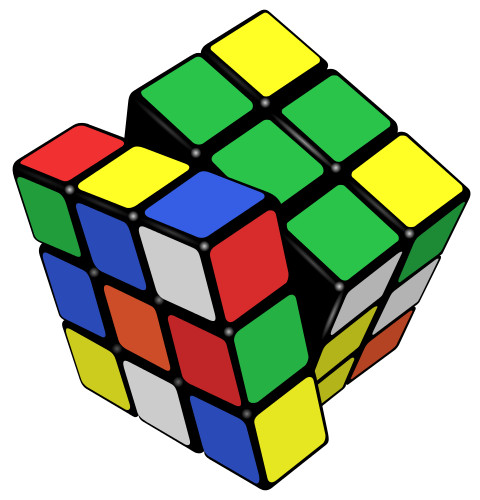
\includegraphics[scale = 0.3]{RubikCube.jpg}
\caption{Rubik’s Cube}
\end{figure}

Dans la première partie, on présentera la structure du programme qu’on a adopté et quelques notions  sur l’algorithmes de recherche. Puis dans la deuxième partie, on analysera nos résultats et expliquera les optimisations du programme et les éventuelles améliorations.


%------------------------------------------------

\section{Implémentation}

~\\\indent
Le projet est composé de deux parties, la programmation et les études sur l’algorithme. Dans un premier temps, on montrera l’utilité de chaque classe pour donner une perspective sur notre programme et on présentera les différents algorithmes qu’on a utilisé par la suite.

\subsection{Structure du programme}

~\\\indent
Le programme est divisé en 4 paquets, \class{Cube} pour modéliser le Rubik’s Cube, \class{Chemin} pour l’algorithme de recherche, \class{Config} pour l’initialisation du programme, enfin \class{Default} pour le test.

\paragraph{\class{Cube.Cube}}
Cette classe modèlise le cube par un tableau d’entier (6 faces de 3 * 3) : \class{int[][][] color}. On utilise, pour une raison de simplicité, les entiers de 0 à 5 pour numéroter les différentes faces. Les constructeurs principaux permettent soit de créer le cube en rentrant les couleurs (sous-entendu leur indice) dans la console d'Eclipse, soit de le créer en lisant un fichier texte. \class{print} et \class{show2D} permettent d'afficher le cube respectivement dans la console sous forme schématique ou dans une fenêtre extérieure comme décrit dans \class{Plan}. Pour tourner le cube, \class{tournerFace} permet de ne tourner que la face de la rotation, tandis que la rotation des 4 faces environnantes se fait avec \class{set}, qui remplace une rangée (ligne ou colonne) par une autre et renvoie la rangée initiale, ce qui permet de faire la rotation pour les 4 faces. Puis on fait appel à \class{tourner} pour une rotation complète en faisant fait tourner une face entre 1 et 3 fois dans le sens trigonométrique, pour avoir sens trigonométrique, demi-tour et sens horaire. Deux comparateurs \class{same} et \class{faceHomogene} permettent de tester respectivement l'égalité de 2 cubes et le bon positionnement d'une face, et seront utiles pour les algorithmes. On y trouvera également des fonctions comme\class{distance}, la fonction heuristique et \class{hashC} pour donner une identifiant unique à chaque configuration. 

\begin{figure}[h]
\centering 
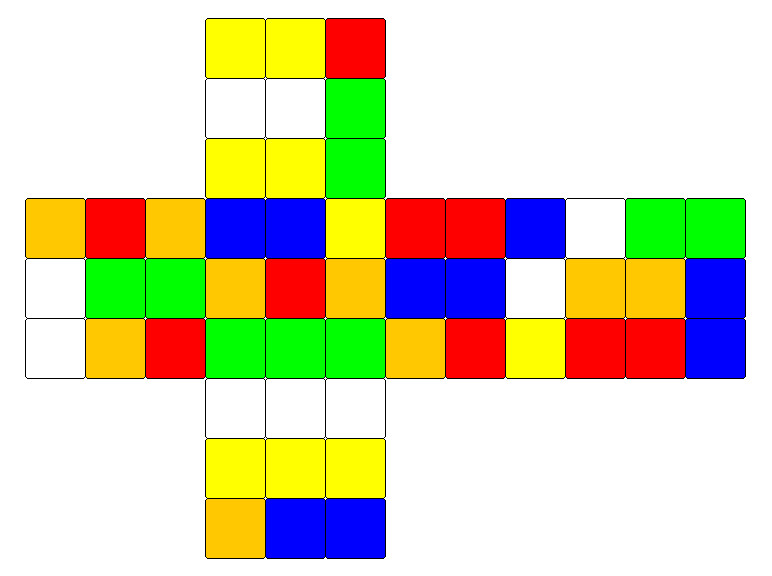
\includegraphics[scale = 0.21]{Plan.jpg}
\caption{Représentation 2D du Rubik’s Cube}
\end{figure}

\paragraph{\class{Cube.Plan}}
Afin de visualiser plus clairement le cube que dans la console, on a utilisé les interfaces graphiques de Java pour dessiner notre cube sur un plan. Une fois que les coordonnées de chaque face sont calculées à la main, il ne reste plus qu’à appeler la méthode \class{paint}. Les couleurs sont rangés dans un tableau colors qui sera repris pour la construction du cube, chaque couleur étant appelée par son indice dans ce tableau, pour plus de facilité. On remarque que ces couleurs sont modifiables pour s’adapter à des cubes exotiques. 

\paragraph{\class{Cube.Coin}}
Cette classe modélise le coin du cube avec trois couleurs et leurs coordonnées (dans le tableau \class{color} du cube). Le champs \class{index} numérote le coin de 0 à 7 selon leurs couleurs (il vaut -1 si cette combinaison de couleurs n’existe pas) et \class{occupied} enregistre la position réelle de ce coin, si les deux valeurs diffèrent, le coin est mal mis. Plusieurs constructeurs sont proposés, le plus utile a pour paramètre un cube et le numéro du coin. Il permet de trouver facilement les couleurs du coin demandé avec un tableau statique \class{realPosition} qui stocke toutes les coordonnées des coins.

\paragraph{\class{Cube.Edge}}
Cette classe est similaire à \class{Coin}, elle modélise les 12 arêtes avec leur deux couleurs, les champs et méthodes sont presque identiques.

\paragraph{\class{Chemin.Chemin}}
Dans cette classe on trouve comme champ important \class{initial}, \class{final} et \class{chemin} qui stocke le cube à tester, le cube final qu’on veut (presque toujours le même) et une liste d’\class{Action} pour y arriver. Comme méthodes, on a utilisé une recherche \class{runFindDFS} pour une DFS limité et \class{runFindIDA} pour laquelle on a le choix entre plusieurs fonctions heuristiques possibles. Plusieurs autres recherches ont été implémentées pour la comparaison. On peut également trouver un champ \class{Time} qui limite le nombre de configurations qu’on visite de façon à interrompre la recherche (pour un nombre de 100 000, il faut préparer quelques secondes).

\paragraph{\class{Chemin.Action}}
Avec deux entiers \class{face} et \class{tour}, cette classe encapsule les rotations  du cube et aussi de défait une action pour revenir à la configuration initiale du cube avec deux méthodes \class{Run} et \class{Rollback}. Il existe une autre classe de même type \class{Disposition} qui implémente une liste d’\class{Action} et qui est beaucoup moins utilisée.

\paragraph{\class{Chemin.ActionComparator}}
Une simple classe implémentant une fonction de comparaison de deux actions afin de construire une queue de priorité dans certaines recherches. 

\paragraph{\class{Config.Distance}}
Dans la suite des algorithmes, nous aurons besoin de calculer les distances pour placer coins et arêtes. Cette classe ne possède que des membres statiques. Ses champs comme \class{distCoin} et \class{distEdge} sont accessibles au moment de la recherche pour calculer la fonction heuristique. Ses méthodes permettent de calculer ces distances ou de les lire dans un fichier.

\paragraph{\class{Config.PatternArray}}
Cette classe est un autre calcul de la distance. On part d’un cube propre et en faisant un parcours en profondeur de 12 étapes maximaux (idéalement) pour essayer de parcourir toutes les sous-configurations possibles et d’enregistrer le chemin minimal dans un support. La méthode \class{calculatePattern} calcule ces valeurs et les enregistre d’abord dans un tableau \class{coin} par exemple, puis dans un fichier binaire, puis \class{readBinaryPattern} les reprend pour les tests dans le futur pour éviter de passer des heures à initialiser le programme.

\paragraph{\class{Test}}
Cette dernière classe comporte tous les tests qu’on utilise pour soit tester le bon fonctionnement d’une module, soit résoudre proprement un Rubik’s Cube et comparer les différentes méthodes.

\subsection{Algorithmes de recherche}

~\\\indent
L’idée principale de la recherche et de partir d’une configuration \class{initial}, de faire une suite d’\class{Action} en comparant à chaque étape si on arrive sur \class{final}. On considère dans ce cas-là chaque configuration du Rubik’s Cube comme un noeud et chaque noeud possède 15 noeuds voisins (on est dans un graphe orienté) ou 18 juste pour le premier noeud où on part. Cette modélisation nous suggère d’utiliser les algorithmes de recherche de plus court chemin dans un graphe.

\paragraph{BFS}
L’idée naïve et naturelle est de faire un parcours en largeur. Cette méthode est impossible d’atteindre l’état final à notre jour puisqu’il faut parcourir dans le pire des cas $18*15^{19}$ noeuds pour trouver une solution. 

\paragraph{DFS limitée}
Une recherche un profondeur peut aller très loin, mais elle ne donne pas forcément une solution optimale. Pour corriger ce défaut, on utilise une limite pour restreindre la profondeur de la recherche. Lorsqu’on ne trouve pas de solution avec la limite donnée, on l’incrémente et continue la recherche. Bien que cette méthode ne diffère pas beaucoup de BFS, elle propose une piste très intéressante, car avec une DFS, le coût de mémoire est proportionnel et non exponentiel à la profondeur, on n’a qu’un cube à faire tourner. 

\paragraph{IDA*}
Comment donc choisir la bonne limite dans l’algorithme précédent ? L’algorithme A* nous donne une autre piste. Avec une fonction heuristique donnant une bonne inférieure de la distance restante, on ne craint plus d’avoir une solution non optimale. Puis une estimation de la distance totale (coût + ce qui reste) permet d’éliminer certains cas, car ils sont trop loin du but. Il est à noter que A* ne donne en général pas une distance minimale puisqu’il s’enfonce sur une piste qu’il croit la meilleure, il est surtout utilisé pour une recherche rapide d’une solution quelconque. Pour que cet algorithme marche, il nous faut une bonne fonction heuristique et on verra tout à l’heure que ces fonctions sont soit inutilisables, soit très coûteuses. Une méthode à la fois facile à implémenter et efficace n’a pas encore été trouvées. Les fonctions heuristiques qu’on a utilisé se trouvent dans la liste suivante: 

\begin{itemize}[noitemsep] % [noitemsep] removes whitespace between the items for a compact look
\item Simple : nombre de coups pour placer une piece
\item Manhattan : distance Manhattan
\item Coin : étapes minimaux pour remettre les 8 coins
\item Arête 1 : remettre les 6 premières arêtes
\item Arête 2 : remettre les 6 autres
\item Pattern : maximum de c, o et e
\end{itemize}

%------------------------------------------------

\section{Analyses}

~\\\indent
Dans cette partie, on retourne vers notre programme lui-même. On expliquera plus en détail les méthodes qu’on a utilisé et les choix qu’on a fait. On présentera également le résultat des différents tests pour faire une comparaison horizontale entre les algorithmes et les fonctions heuristiques et on essayera de comprendre comment ces fonctions permmetten d’avoir un effet si important sur notre recherche.

\subsection{Fonction heuristique}

~\\\indent
Pour utiliser l’algorithme IDA*, il nous faut une fonction heuristique ou un estimateur de distance. Les conditions nécessaires et suffisantes d’utilisation d’une telle fonction sont prouvées dans la section précédente. Ici, on va comparer de diverses fonctions et essayer de comprendre en quoi elles sont différentes.

\begin{table}[htbp]
\centering
\begin{tabular}{cccc}
\hline
\rowcolor{blue!20} \rule{0pt}{12pt} \textbf{Profondeur} & \textbf{Simple\textsuperscript{1} } & \textbf{Manhattan}\textsuperscript{1} & \textbf{Pattern\textsuperscript{1}}\\
\hline
3 & 0 & 3 & 0 \\
4 & 2 & 5 & 0 \\
5 & 20 & 26 & 0 \\
6 & 223 & 135 & 0  \\
7 & 1380 & 215 & 0 \\
8 & - & 1118 & 1 \\
9 & - & - & 13 \\
10 & - & - & 79 \\
11 & - & - & 1161 \\
12 & - & - & 7309 \\
\hline
\multicolumn{4}{l}{\small{1. La signification se trouve dans la section précédente}} \\
\hline
~\\
\end{tabular}
\caption{Temps (en ms) de la recherche (estimateur)}
\end{table}

\begin{table}[htbp]
\centering
\begin{tabular}{cccc}
\hline
\rowcolor{blue!20} \rule{0pt}{12pt} \textbf{Profondeur} & \textbf{Coins\textsuperscript{1} } & \textbf{Arêtes 1}\textsuperscript{1} & \textbf{Arêtes 2\textsuperscript{1}}\\
\hline
4 & 0 & 0 & 2 \\
5 & 2 & 0 & 90 \\
6 & 8 & 0 & 220  \\
7 & 38 & 1 & 1256 \\
8 & 123 & 13 & - \\
9 & 220 & 144 & - \\
10 & 1855 & 339 & - \\
11 & - & 1108 & - \\
\hline
\multicolumn{4}{l}{\small{1. La signification se trouve dans la section précédente}} \\
\hline
~\\
\end{tabular}
\caption{Temps (en ms) de la recherche (Pattern)}
\end{table}

\indent
On constate que plus la fonction heuristique donne une grande valeur (Distance simple : 3 ; Manhattan : 6 ; Pattern : 9), plus on va loin dans la recherche. Ce qui est dû à notre algorithme de recherche qui recalcule la limite de profondeur à partir de la distance minimale qu’on estime. Cependant, la différence entre Arête 1 et 2 semble inexpliquable puisqu’elle sont symétrique a priori.

\subsection{Pattern Database}

~\\\indent
Comment enregistrer les résultats une fois qu’on les a calculés ? Un tableau a l’air d’être plus adaptée à ce genre de situation, car les clés sont des entiers consécutifs et elles ne dépassent pas la taille limite des entiers ($2^{32}$). Il suffit de créer un tableau de taille suffisamment grande.

\begin{itemize}[noitemsep] % [noitemsep] removes whitespace between the items for a compact look
\item Coins :  $8! * 3^7 = 88179840$ cas
\item Arêtes : $\frac{12!}{6!}*2^6$ cas (idem pour l’autre partie d’arêtes)
\end{itemize}

On constate bien que le nombre de cas ne dépasse pas la capacité de JVM et l’utilisation d’un tableau permet à la fois d’économiser le coût en mémoire et en temps aussi puisque l’accès aux valeurs ne coût que quelques opérations élémentaires. 

Malgré le nombre de cas limité, il nous faut toujours trouver un moyen de stocker les résultats. En comparant les différentes méthodes, nous avons adopté une méthode non optimale, mais largement acceptable dans notre cas. Voyons une breve comparaison :

\begin{itemize}[noitemsep] % [noitemsep] removes whitespace between the items for a compact look
\item Texte :  $(88179840 + 42577920 * 2) * 8 = 173$ Mb
\item Binaire avec 1 byte par valeur : $173$ Mb
\item Binaire avec 4 bits par valeur : $87$ Mb
\end{itemize}

Nous avons choisi finalement le fichier binaire en utilisant la classe \class{DataOutputStream} pour stocker notre valeur, parce que l’enregistrement bit par bit est difficile à réaliser et peut ralentir le programme si c’est mal implémenté, et par rapport au fichier texte, on n’a plus besoin de faire une conversion de \class{String} vers \class{Byte}, ce qui fait gagner du temps. 

Cependant, pour générer tous les cas possibles, il faut faire un parcours en largeur d’une profondeur de 10 (car le nombre de coups maximal pour remettre ces 3 sous-parties est de 11). La durée est d’autant plus longue qu’on augmente la profondeur. Sur notre ordinateur de test, on a passé 540 secondes pour faire un parcours de profondeur 7. Il faudra donc une semaine pour avoir une base de données complètes.

\subsection{Algorithmes de recherche}

~\\\indent
Dans la section précédente, nous avons présenté les 3 algorithms testés. Pour se donner une idée de la performance de chaque algorithme, on pourra jeter un coup d’oeil sur le résultat d’un test de comparaison entre les différentes méthodes. La fonction heuristique choisie est celle qui utilise Pattern Database.

\begin{table}[htbp]
\centering
\begin{tabular}{ccccc}
\hline
\rowcolor{blue!20} \rule{0pt}{12pt} \textbf{Profondeur} & \textbf{BFS} & \textbf{DFS}\textsuperscript{1} & \textbf{IDA*} &  \textbf{IDA* (PQ)\textsuperscript{2}}\\
\hline
1 & 0 & 0 & 0 & 0  \\
%\hline
2 & 0 & 0 & 0 & 0 \\
%\hline
3 & 0 & 5 & 0 & 0 \\
%\hline
4 & 5 & 187 & 0 & 0 \\
%\hline
5 & 687 & 466 & 0 & 0 \\
%\hline
6 & 7965 & 1142 & 0 & 0  \\
%\hline
7 & - & - & 0 & 0 \\
%\hline
8 & - & - & 5 & 8 \\
%\hline
9 & - & - & 14 & 19 \\
%\hline
10 & - & - & 81 & 111 \\
%\hline
11 & - & - & 956 & 868 \\
%\hline
12 & - & - & 5621 & 5363 \\
%\hline
13 & - & - & 13513 & 8879 \\
%\hline
14 & - & - & (31488)\textsuperscript{3} & (34488)\textsuperscript{3} \\
\hline
\multicolumn{5}{l}{\small{1. DFS avec une profondeur limité}} \\
\multicolumn{5}{l}{\small{2. Avec une queue de priorité pour trier les chemins}} \\
\multicolumn{5}{l}{\small{3. Cette valeur est calculée avec moins de 5 essais}} \\
\hline
~\\
\end{tabular}
\caption{Temps (en ms) de la recherche (algorithme)}
\end{table}

\indent
On constate que l’utilisation de la queue de priorité n’a pas amélioré la vitesse de recherche de IDA*, ce qui est dû principalement à la maintenance de la queue. Quant à sa performance générale, ce résultat n’est point surprenant. Pour une solution de moins de 8 étapes (ce qui correspond au niveau de notre Pattern Database, c’est-à-dire qu’il possède toutes les configurations d’une distance inférieure ou égale à 8), à chaque appel récursif, on est sûr de s’approcher plus de l’état final, ceci dit qu’on a toujours au moins un chemin pour faire diminuer la distance. Et comme la distance initiale est inférieure ou égale à 8, la solution sera trouvé très vite. Au-delà de 8 étapes, on constate qu’il y a une augmentation de temps comme dans les autres cas, cela vient du fait qu’on ne plus pas distinguer par exemple deux distances 9, car dans ces cas-là la distance n’est qu’une borne inférieure (la solution peut aller jusqu’à 20 étapes, mais on ne peut pas savoir), cela brouille la piste de recherche et on est obligé d’étudier beaucoup de cas comme s’ils étaient un bon chemin. On pourrait comprendre cet algorithme comme une translation (sur l’axe de profondeur) d’une distance imposée par le niveau de Pattern Database.

\subsection{Conclusion}

~\\\indent
Bien que le résultat précédent n’est pas suffisant pour résoudre un cube quelconque, il nous donne une piste de l’amélioration : agrandir Pattern Database et améliorer la classe \class{Cube} pour accélérer le parcours. Plus la base de données est complète, plus on choisit la bonne direction. On constate néanmoins que ce qu’on fait c’est de gagner du temps en sacrifiant de l’espace. La complexité du problème reste toujours la même. Rien n’interdit aujourd’hui de résoudre complètement le Rubik’s Cube, mais cela demandera une optimisation encore plus poussée que celle présenté dans ce rapport et surtout un ordinateur plus puissant.

%------------------------------------------------
\phantomsection
\section*{Annexe} % The \section*{} command stops section numbering

\addcontentsline{toc}{section}{Annexe} % Adds this section to the table of contents

~\\\indent
Dans cet annexe, vous trouvez une explication en détail de la mise en route de notre programme.

\paragraph{Initialisation}

\paragraph{Entrée des données}

\paragraph{Recherche de la solution}

\paragraph{Autres test}

\end{document}